Below are the results of the low pass filter. The measured frequencies and amplitudes are then plotted on a bode plot.

\begin{adjustwidth}{-2.5 cm}{-2.5 cm}\centering\begin{threeparttable}[!htb]
        \scriptsize
        \begin{tabular}{lrrrrr}\toprule
            \textbf{Input Voltage(in V)} & \textbf{Output Voltage(in V)} & \textbf{Phase(in deg)} & \textbf{Frequency(in Hz)} & \textbf{Amplitude(in dB)} \\\midrule
            10.1                         & 10                            & -0.36                  & 50                        & 20.00                     \\
            10.1                         & 10                            & -0.36                  & 100                       & 20.00                     \\
            10.1                         & 10                            & -2.59                  & 200                       & 20.00                     \\
            10.2                         & 10                            & -6.49                  & 500                       & 20.00                     \\
            10.4                         & 10.1                          & -11.8                  & 1000                      & 20.09                     \\
            10.9                         & 10                            & -23                    & 2000                      & 20.00                     \\
            12.2                         & 8                             & -47.4                  & 5000                      & 18.06                     \\
            11.8                         & 5.04                          & -64                    & 10000                     & 14.05                     \\
            12.4                         & 2.8                           & -75.3                  & 20000                     & 8.94                      \\
            11.8                         & 1.14                          & -82.8                  & 50000                     & 1.14                      \\
            11.8                         & 0.596                         & -84.6                  & 100000                    & -4.50                     \\
            \bottomrule
        \end{tabular}
        \caption{The measured frequencies and amplitudes from the low pass filter.}\label{tab: }
    \end{threeparttable}\end{adjustwidth}


\begin{figure}[H]
    \centering
    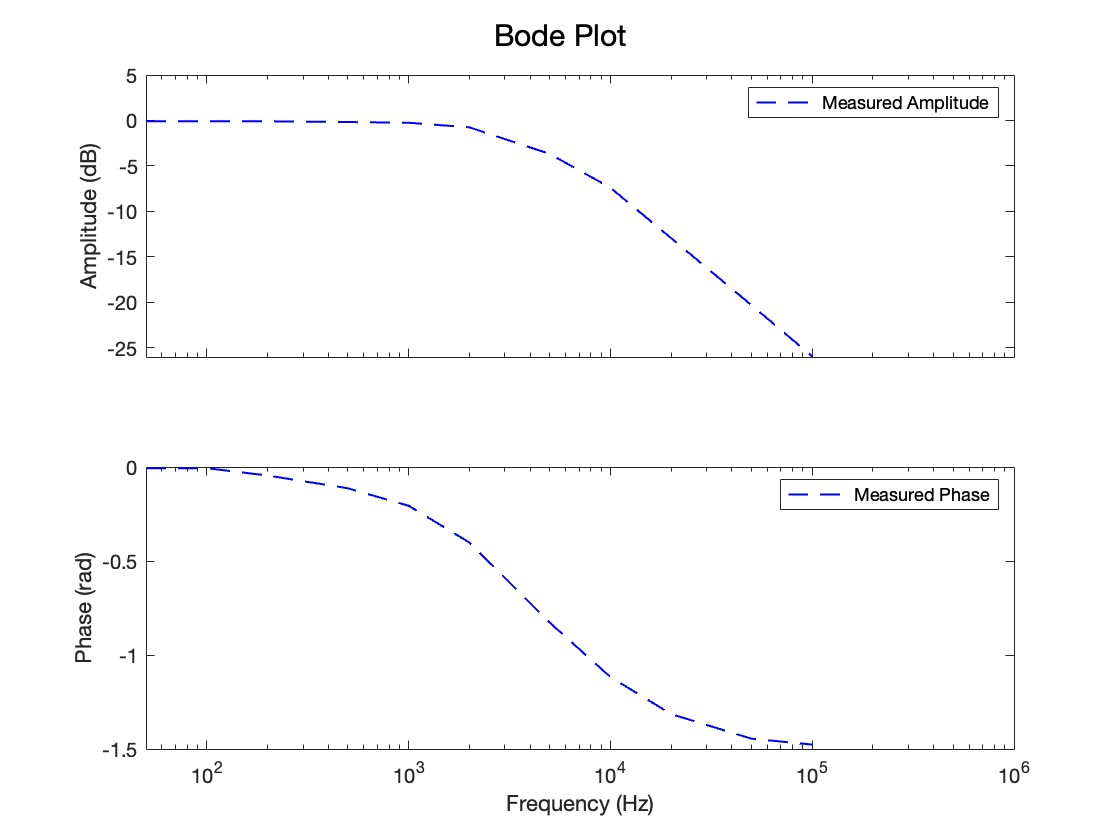
\includegraphics[scale=0.3]{images/bode_plot_low_pass_measured.jpg}
    \caption{Bode plot of measured frequencies, amplitudes and phase shifts of the low pass filter.}
\end{figure}

To draw the bode plot of the calculated amplitudes and phase, we use the following formulas:
$|\underline{A}| = \frac{1}{\sqrt{1 + (\omega RC)^2}} \text{ and } \phi = -\arctan(\omega RC)$


\begin{figure}[H]
    \centering
    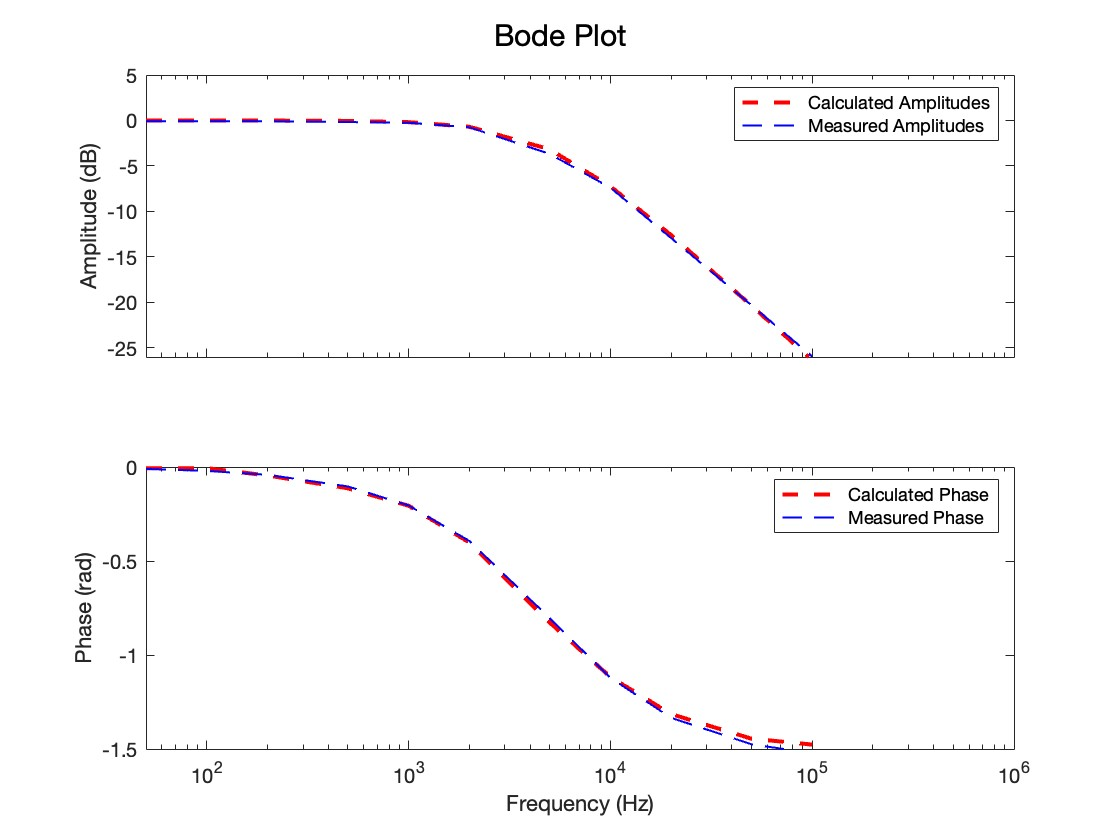
\includegraphics[scale=0.3]{images/bode_plot_low_pass_calculated.jpg}
    \caption{Bode plot of calculated amplitudes and phase shifts of the low pass filter using measured frequencies.}
\end{figure}



The calculated cutoff frequency can be obtained by the following relation for the low pass filter circuit:
\begin{equation}
    f_{-3dB} = \frac{1}{2\pi RC}
\end{equation}

Where the cutoff frequency becomes

\begin{equation}
    f_{-3dB} = \frac{1}{2\pi (22\cdot 10^3\Omega)\cdot(1\cdot 10^{-9}{F})} = 4822.8{Hz}
\end{equation}

\begin{figure}[H]
    \centering
    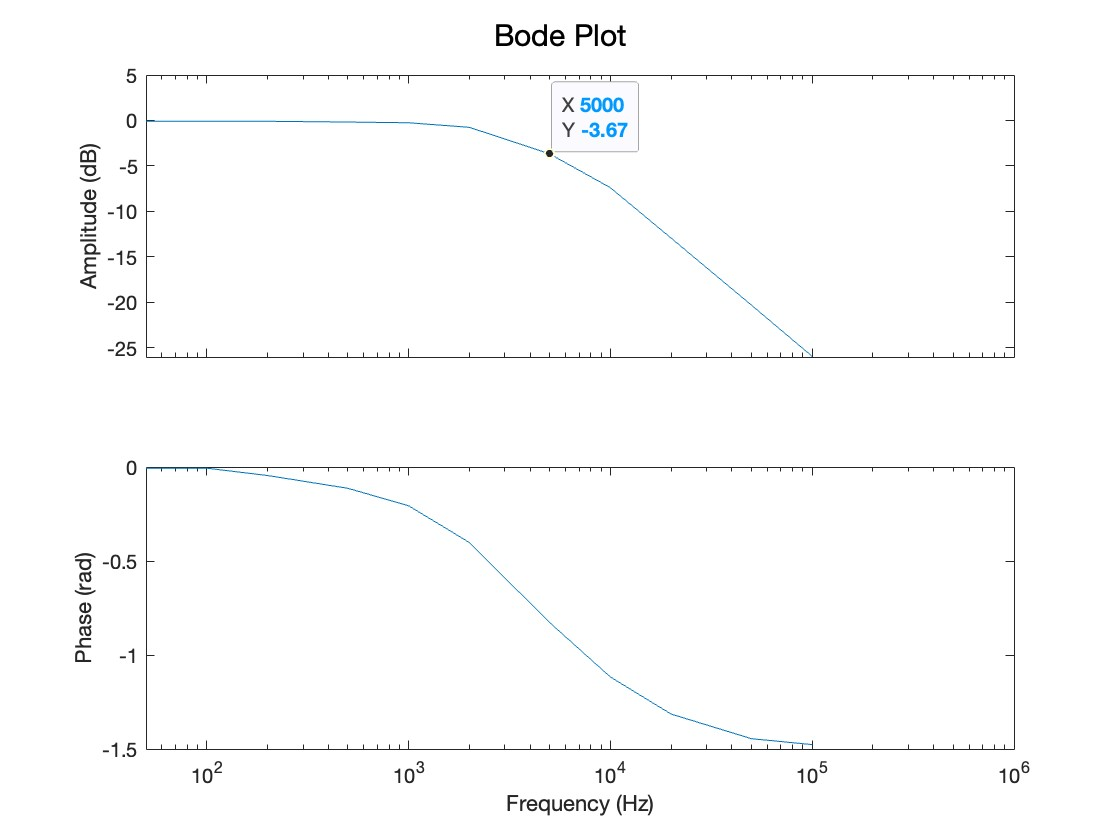
\includegraphics[scale=0.3]{images/bode_plot_low_pass_measured_cutoff.jpg}
    \caption{Bode plot of measured amplitudes and phase shifts of the low pass filter using measured frequencies.}
\end{figure}
Comparing against the cutoff frequency of the measured wave, we see that it is quite within range of the calculated cutoff frequency of 4822.8{Hz}.

To find the gradient of $|A|$, we find the derivative of the magnitude of the transfer function:
\begin{equation}
    \frac{d|A|}{df} = \frac{d}{df}\left(\frac{1}{\sqrt{1+(\omega RC)^2}}\right) = \frac{-(2*(2\pi fRC) * (2\pi RC))}{2(1+(2\pi fRC)^2)^{\frac{3}{2}}} = -\frac{(4\pi^2R^2C^2)f}{(1+4\pi^2f^2R^2C^2)^{\frac{3}{2}}}
\end{equation}

Taking the limit of $|A| = \frac{1}{\sqrt{1+(\omega RC)^2}}$ and the limit of $\phi = -\tan^{-1}(\omega RC)$, we get the following table:

\begin{table}[!htp]\centering
    \scriptsize
    \begin{tabular}{lrrrr}\toprule
        Case             & Behaviour of f   & Amplitude            & Phase         \\\midrule
        $f \gg f_{-3dB}$ & $f \to \infty$   & $0$                  & $-90^{\circ}$ \\
        $f = f_{-3dB}$   & $f \to f_{-3dB}$ & $\frac{1}{\sqrt{2}}$ & $-45^{\circ}$ \\
        $f \ll f_{-3dB}$ & $f \to 0$        & $1$                  & $0^{\circ}$   \\
        \bottomrule
    \end{tabular}
    \caption{The behavior of the frequency depending on the case of $f_{-3dB}$}\label{tab: }
\end{table}
By this table we can infer that when the frequency is under that of the cutoff frequency, the ratio is one - the filter should ideally let the signal pass through without attenuation and any phase shift.
We can also infer that when the frequency is that of the cut-off frequency, we get the amplitude and the phase of the corner frequency.
Lastly, we can infer that when the frequency is way greater than the cut-off frequency, the amplitude is zero and the phase is $-90^{\circ}$.